\section*{Listing des fichiers}
\begin{itemize}
	\item \verb+casn.txt+ avec (n $\in$ [0..6]) : les fichiers générés par l'exécution du code Java
	\item \verb+Mesure.java+ et \verb+Methodes.java+ les fichiers source requis pour la génération de tous les fichiers de données
	\item \verb+tpog.plot+ : unique fichier de commande gnuplot permettant la génération de tous les graphiques en une seule exécution
\end{itemize}

\section*{1 Gnuplot}

Voir les fichiers :
\begin{itemize}
	\item \verb+fichier.txt+
	\item \verb+graphique.png+
	\item \verb+tpog.plot+
\end{itemize}

\section*{2 Comparaisons de méthodes Java et d'algorithmes fait maison}

\subsection*{2.1 Influence sur les données}
~\\

\textbf{Q1.}
~\\
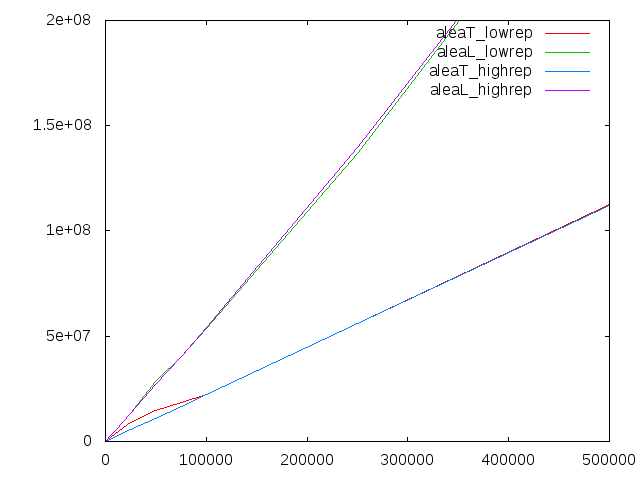
\includegraphics[height=12cm, width=\textwidth]{../lin_aleaTL.png}
~\\
Nous constatons que la méthode \verb+aleaT+ est plus rapide que la méthode \verb+aleaL+, quelque soit le nombre de répétitions.
~\\

\textbf{Q2.}
~\\
Le nombre de répétitions n'a quasiment pas d'influence sur les courbes.
~\\

\textbf{Q3.}
~\\
//TODO
~\\

\textbf{Q4.}
~\\
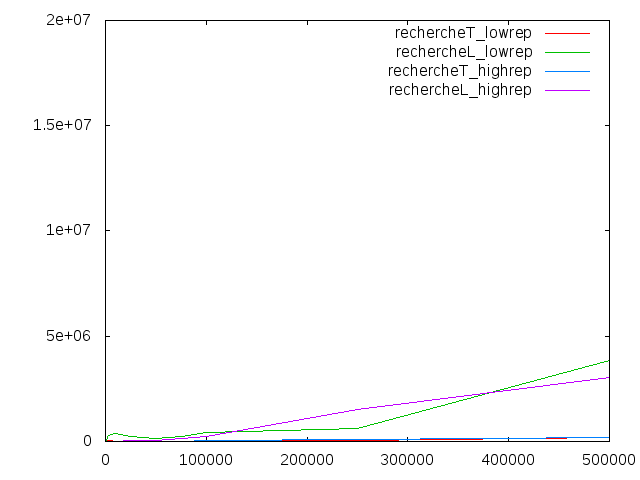
\includegraphics[height=12cm, width=\textwidth]{../lin_rechercheTL.png}
~\\
Nous constatons que la méthode \verb+rechercheT+ est plus rapide que la méthode \verb+rechercheL+, quelque soit le nombre de répétitions.
~\\

\textbf{Q5.}
~\\
Le nombre de répétitions a une petite influence sur les courbes.
~\\

\textbf{Q6.}
~\\
Sur les huit mesures précédentes, nous constatons que les opérations sur les tableaux sont plus rapides que sur les listes.
~\\

\textbf{Q7.}
~\\
Les variations d'influence du nombre de répétitions de la mesure s'explique par la variation de la complexité des deux algorithmes :
\begin{itemize}
	\item \verb+alea()+ : place des entiers de 0 à size - 1 dans un ordre aléatoire
	\item \verb+recherche(int e)+ : recherche l'entier e dans la structure de données
\end{itemize}
La complexité d'\verb+alea+ est constante, alors que celle de \verb+recherche+ dépend de la disposition des entiers dans la structure. Voilà pourquoi la répétition a une influence dans \verb+recherche+ et n'en a pas dans \verb+alea+.
~\\

\textbf{Q8.}
~\\
Nous pouvons conclure qu'il faut choisir un nombre faible de répétitions (même si ce nombre n'a pas d'influence quand la complexité de l'algorithme étudié est constante.
~\\

\subsection*{2.2 Recherches de minima}
~\\

\textbf{Q9.}
~\\
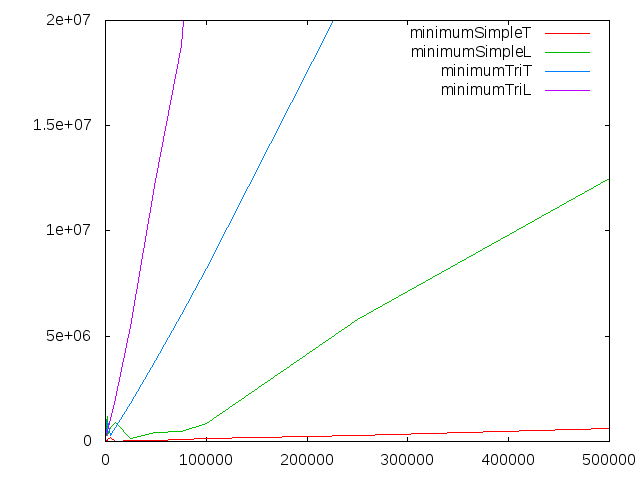
\includegraphics[height=12cm, width=\textwidth]{../lin_minimumTL.png}
~\\
Nous constatons que les méthodes \verb+minimumSimpleT+ et \verb+minimumTriT+ sont plus rapides que les méthodes \verb+minimumSimpleL+ et \verb+minimumTriL+, quelque soit le nombre de répétitions.
~\\

\textbf{Q10.}
~\\
Nous pouvons dire que le nombre de répétitions fait beaucoup varier l'efficacité de ces deux structures de données.
~\\

\textbf{Q11.}
~\\
Nous pouvons dire qu'il est plus efficace de ne pas trier le tableau ou la liste avant d'en rechercher le minimum.
~\\

\section*{3 Comparaisons des fonctions de référence}

\subsection*{3.1 Vue d'ensemble}
~\\

\textbf{Q12.}
~\\
Cela n'a pas été facile. Il a fallu adapter notre tableau de tailles pour ne pas avoir des valeurs infinies et l'échelle de notre graphique pour voir les courbes.
~\\

\textbf{Q13.}
~\\
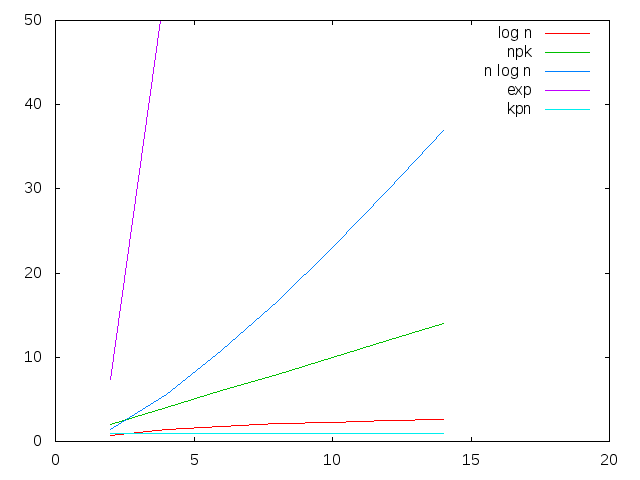
\includegraphics[height=12cm, width=\textwidth]{../lin_ref.png}
~\\
Nous pouvons déduire que la fonction exponentielle croît beaucoup plus vite que les autres fonctions de référence.
~\\

\textbf{Q14.}
~\\
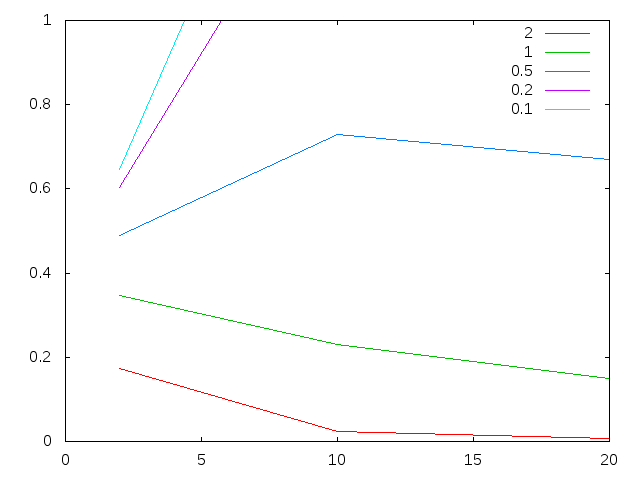
\includegraphics[height=12cm, width=\textwidth]{../lin_lognepsi.png}
~\\

\textbf{Q15.}
~\\
Plus $\varepsilon$ est grand, plus $\frac{log n}{n^\varepsilon}$ est petit.\\
=> $\lim\limits_{\substack{x \rightarrow +\infty}} (\frac{log n}{n^\varepsilon})$ = 0 \\
=> \fbox{$log n$ = O($n^\varepsilon$) ($\varepsilon$ > 0)}
~\\

\textbf{Q16.}
~\\
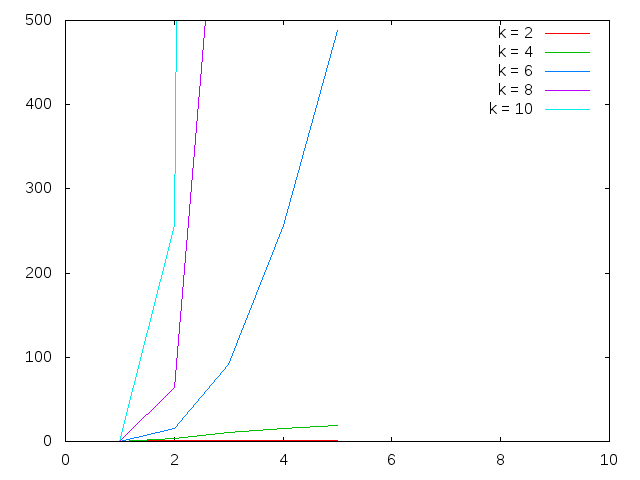
\includegraphics[height=12cm, width=\textwidth]{../lin_npk2pn.png}
~\\

\textbf{Q17.}
~\\
\fbox{$n^k$ = $\Omega(2^n)$}
~\\

\section*{4 Détermination expérimentale de la complexité d'un algorithme}
~\\

\textbf{Q18.}
~\\
L'algorithme codé par les deux méthodes mystères est une méthode de tri basée sur des renversements de portions de tableaux/listes.
~\\

\textbf{Q19.}
~\\
Donnons le pseudo-code de cet algorithme : \\

\verb+soit t la structure à trier et n sa longueur+ \\
\verb+pour i allant de 0 à n - 1 faire+ \\
\verb+soit p la position du minimum dans t[i..n-1]+ \\
\verb+renverser les éléments de t entre les positions p et n - 1+ \\
\verb+(t[n-1] contient l'élément minimal de t[i..n-1])+ \\
\verb+renverser les éléments de t entre les positions i et n - 1+ \\
\verb+(t[i] contient l'élément minimal de t[i..n-1])+ \\
\verb+fin pour+ \\

Chaque tour de boucle est caractérisé par 3 étapes : la recherche du minimum, un renversement, et un autre renversement

Ses cas extrêmes sont :
\begin{description}
	\item[Meilleur des cas :] à chaque tour de boucle, l'élément minimum se trouve en dernière position. Le premier renversement ne fera donc rien.
	\item[Pire des cas :] la structure est triée par ordre croissant. Ainsi, à chaque tour de boucle, l'indice de boucle est l'indice du minimum de la structure. Le premier renversement se fait donc toujours sur toute la partie du tableau structure (comme le deuxième).
\end{description}
~\\
Cet algorithme est en $\Theta(n^2)$.
~\\

